% ============================================================
%  CHAPTER 1: INTRODUCTION
% ============================================================

\chapter{INTRODUCTION}
\label{chap:introduction}

\section{Background of VPN Technology}
\label{sec:vpn_background}

A Virtual Private Network (VPN) is an indispensable network security technology designed to establish a protected, encrypted communications channel across an inherently untrusted public intermediate network, such as the global Internet~\cite{stallings2022cryptography}. Originally conceptualized to interconnect geographically distributed corporate offices and provide secure remote access for telecommuting personnel, VPN architectures have evolved into the foundational defense mechanism for modern enterprise communications, cloud perimeter defense, critical infrastructure monitoring, and personal mobile privacy~\cite{menezes1996handbook,rfc4301}.

At its core, a VPN creates a virtual point-to-point link between two endpoints: a client terminal (e.g., an Android mobile smartphone, a desktop workstation) and a network security gateway (e.g., a dedicated hardware firewall, a Linux tunneling daemon). To achieve this, the underlying system encapsulates raw Layer~3 (Network layer) Internet Protocol (IP) datagrams within an outer transport protocol, encrypts the inner payload using robust symmetric cryptography, and authenticates the integrity of the transmission against adversary interception and manipulation~\cite{ferguson2010cryptography}. When an application on the client device issues an outbound network connection, the operating system routes the resulting raw IP packets not directly to the local physical network adapter (such as a public Wi-Fi access point or a cellular radio interface), but rather to a specialized virtual network interface. In Linux and Unix environments, this virtual interface is implemented via the TUN (network tunnel) driver~\cite{donenfeld2017wireguard}, whereas in modern mobile ecosystems such as Android, it is exposed through the managed \texttt{android.net.VpnService} framework~\cite{android_vpnservice_docs}.

Once captured by the virtual interface, the client tunneling software encrypts the payload, wraps it in transport framing (typically Transmission Control Protocol [TCP] or User Datagram Protocol [UDP]), and dispatches it over the physical network interface to the remote VPN server. Upon receiving the outer frame, the VPN server performs cryptographic authentication and decryption, strips the encapsulation header, assigns or verifies the client's internal virtual IP address, and injects the original cleartext IP packet into its local routing subsystem. Through Network Address Translation (NAT) and packet masquerading, the server dispatches the packet toward its ultimate destination on the public Internet or a private corporate intranet~\cite{ikram2016measuring}.

The fundamental security objectives delivered by a robust VPN implementation comprise:
\begin{enumerate}[label=(\roman*)]
    \item \textbf{Confidentiality}: Ensuring that intermediate network observers, internet service providers (ISPs), rogue wireless access points, and nation-state surveillance systems cannot inspect the plaintext content of transmitted packets.
    \item \textbf{Data Integrity}: Guaranteeing that data cannot be altered, injected, or truncated in transit without immediate detection and rejection by the recipient.
    \item \textbf{Endpoint Authentication}: Establishing mutual cryptographic proof of identity between the connecting client and the serving gateway prior to data exchange.
    \item \textbf{Anti-Replay Defense}: Preventing malicious adversaries from capturing valid encrypted frames and re-transmitting them later to trigger unauthorized state changes or resource exhaustion.
    \item \textbf{Traffic Flow Confidentiality}: Masking the true origin, destination endpoints, and packet patterns of user traffic from external observers.
\end{enumerate}

\section{Network Privacy and Secure Mobile Communication}
\label{sec:network_privacy_mobile}

Mobile smart devices operating on the Android platform have become the primary computing endpoints for enterprise productivity, confidential communications, banking, healthcare, and governance worldwide. By their very nature, mobile devices operate in perpetually dynamic, untrusted radio environments. Throughout a typical working day, a smartphone transitions continuously across heterogeneous network perimeters, including residential broadband Wi-Fi, open public Wi-Fi hotspots in airports and hospitality venues, and carrier-grade 4G/5G cellular towers~\cite{mavroudis2017touchlog}.

Public and semi-public wireless networks represent hostile threat environments. Rogue access points (such as Evil Twin configurations and Wi-Fi Pineapple deployments) frequently perform Address Resolution Protocol (ARP) spoofing, DNS hijacking, and SSL/TLS stripping attacks to intercept client communications~\cite{kahn2021vpn}. Furthermore, untrusted Internet Service Providers and cellular telecommunications operators routinely collect, inspect, and monetize user traffic metadata, including DNS resolution logs, destination IP addresses, and packet timing signatures. While modern application protocols increasingly deploy Transport Layer Security (TLS~1.3)~\cite{rfc8446}, application-layer encryption alone fails to conceal critical metadata: Server Name Indication (SNI) extensions, destination IP headers, and packet size distributions remain visible to intermediate network observers.

Consequently, operating system-level VPN encapsulation serves as the primary line of defense on mobile devices. By enforcing a full-tunnel configuration (\texttt{0.0.0.0/0}), the mobile operating system routes all outbound application datagrams---including operating system background telemetry, ICMP diagnostic traffic, and raw UDP Domain Name System (DNS) queries---exclusively through the encrypted virtual tunnel. This effectively shields the user's digital footprint behind the gateway's public IP address and prevents local eavesdroppers from gleaning any insight into user activity.

\begin{figure}[htbp]
  \centering
  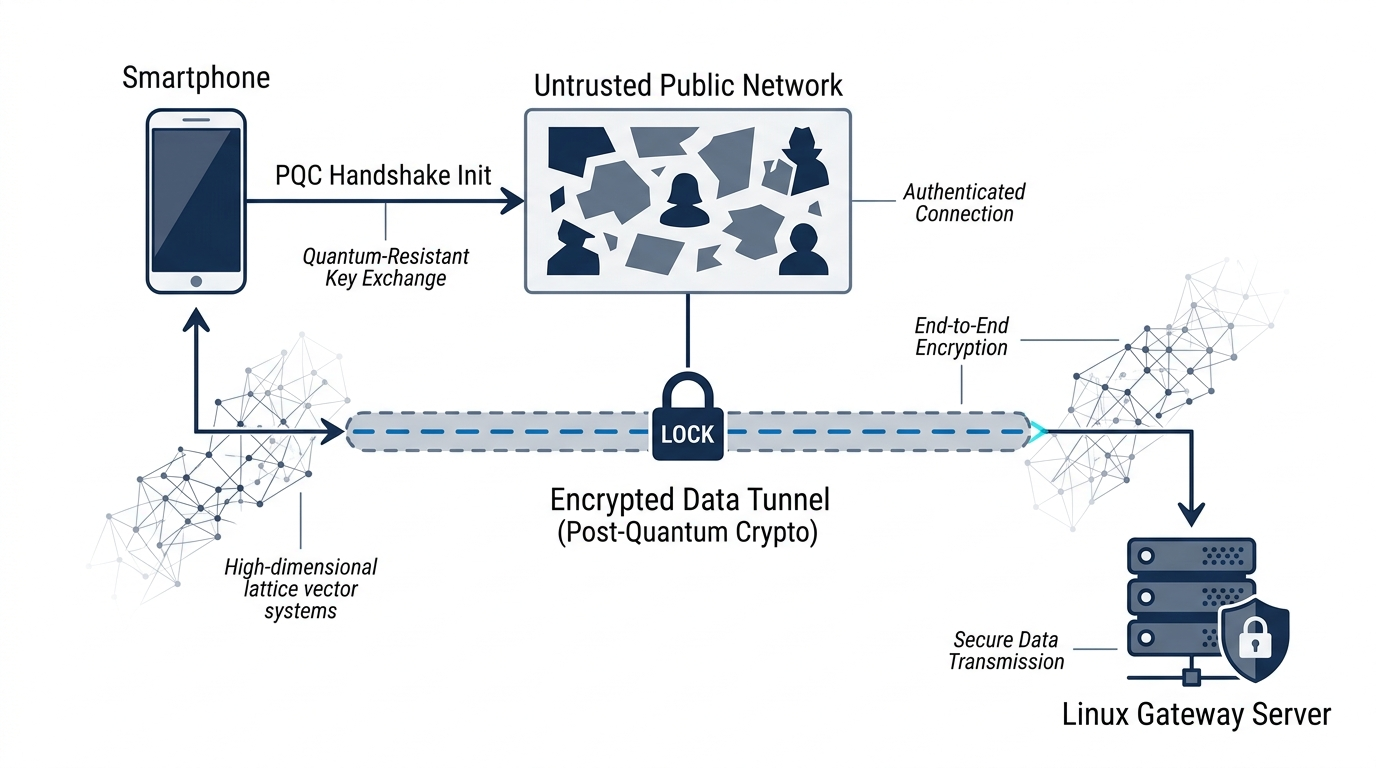
\includegraphics[width=0.92\linewidth,height=0.45\textheight,keepaspectratio]{figures/vpn_cover_graphic.jpg}
  \caption{Conceptual Overview of Mobile VPN Tunneling across Untrusted Public Networks to a Secure Gateway.}
  \label{fig:vpn_cover_overview}
\end{figure}

\section{Evolution of VPN Architectures}
\label{sec:vpn_evolution}

The architectural design of virtual private networking has undergone continuous paradigm shifts across the past three decades, driven by escalating threat capabilities, hardware throughput enhancements, and mobile deployment constraints.

\subsection{First-Generation Protocols: PPTP and L2TP/IPsec}
The earliest widespread tunneling implementation, the Point-to-Point Tunneling Protocol (PPTP), developed in the late 1990s, relied on Microsoft Point-to-Point Encryption (MPPE) and MS-CHAPv2. PPTP suffered from catastrophic architectural vulnerabilities, including trivial credential recovery via offline dictionary attacks and vulnerability to passive eavesdropping. Its successor, Layer 2 Tunneling Protocol combined with IPsec (L2TP/IPsec)~\cite{rfc4301}, separated tunneling from encryption, leveraging Internet Key Exchange (IKEv1) and Triple-DES/AES. While cryptographically sound, L2TP/IPsec exhibited severe limitations on mobile networks: double encapsulation incurred heavy MTU overhead, and intermediate Network Address Translators routinely blocked IPsec's native protocol numbers (IP protocol 50 [ESP] and 51 [AH]), necessitating complex UDP encapsulation workarounds (NAT-Traversal on UDP port 4500).

\subsection{Second-Generation Protocols: OpenVPN and SSL/TLS Tunneling}
OpenVPN revolutionized secure remote access by implementing user-space tunneling over standard OpenSSL TLS sessions~\cite{openvpn2024spec}. Operating across either TCP (typically port 443, mimicking web traffic) or UDP, OpenVPN provided exceptional NAT traversal, highly configurable cipher negotiation, and granular routing options. However, OpenVPN suffers from substantial architectural drawbacks on mobile platforms: its user-space codebase exceeds 100,000 lines of complex C code, resulting in an expansive attack surface. Furthermore, the protocol demands frequent context switching between kernel space and user space across the TUN interface and the network socket, resulting in significant battery drain and elevated packet latency on mobile CPUs.

\subsection{Third-Generation Protocols: WireGuard and Modern Kernel Tunnels}
In 2017, Jason Donenfeld introduced WireGuard~\cite{donenfeld2017wireguard}, an opinionated, minimalist network tunnel engineered directly inside the Linux kernel. With a codebase of under 4,000 lines, WireGuard replaced dynamic cipher negotiation with strict ``cryptographic opinionation,'' relying exclusively on Noise Protocol Framework handshakes, Curve25519 for Diffie-Hellman key exchange, ChaCha20-Poly1305 for authenticated encryption, and BLAKE2s for hashing. WireGuard demonstrated that modern VPNs could achieve near line-rate speeds with minimal CPU utilization.

\subsection{The Emerging Fourth Generation: Post-Quantum Cryptographic VPNs}
Despite the cryptographic elegance of WireGuard and TLS~1.3, all mainstream contemporary VPN architectures share a fatal common denominator: their key-exchange mechanisms rely strictly on classical asymmetric mathematical problems---specifically, the Integer Factorization Problem (RSA) or the Discrete Logarithm Problem over finite fields and elliptic curves (Diffie-Hellman, ECDH/Curve25519)~\cite{diffie1976new,rivest1978method,koblitz1987elliptic}. As established in quantum complexity theory, every single one of these mathematical foundations collapses in the presence of a Cryptographically Relevant Quantum Computer (CRQC)~\cite{shor1994algorithms}. Consequently, the fourth generation of VPN architecture must transition toward lattice-based, post-quantum cryptographic primitives capable of withstanding both classical and quantum cryptanalysis.

\begin{table}[htbp]
  \centering
  \small
  \caption{Evolutionary Comparison of Dominant VPN Architectural Paradigms.}
  \label{tab:vpn_evolution_comparison}
  \begin{tabular}{@{}P{2.4cm}P{2.6cm}P{2.8cm}P{2.8cm}P{3.2cm}@{}}
    \toprule
    \textbf{Protocol} & \textbf{Key Exchange} & \textbf{Data Encryption} & \textbf{Mobile Fit} & \textbf{Quantum Security} \\
    \midrule
    \textbf{PPTP} & MS-CHAPv2 (DES) & MPPE (RC4 128-bit) & Deprecated; poor roaming & Broken classically \\
    \textbf{IPsec (IKEv2)} & DH Groups / ECDH & AES-CBC / AES-GCM & Moderate; complex kernel stack & Completely vulnerable to Shor's algorithm \\
    \textbf{OpenVPN} & TLS (RSA / ECDHE) & AES-CBC / AES-GCM & High battery drain; user-space context switches & Completely vulnerable to Shor's algorithm \\
    \textbf{WireGuard} & Noise IK (Curve25519) & ChaCha20-Poly1305 & Outstanding speed; kernel resident & Completely vulnerable to Shor's algorithm \\
    \textbf{QuantumSafe VPN} & \textbf{ML-KEM-1024 (FIPS 203)} & \textbf{AES-256-GCM (FIPS 197)} & \textbf{Engineered for Android VpnService} & \textbf{Quantum-Safe (NIST Security Category 5)} \\
    \bottomrule
  \end{tabular}
\end{table}

\section{Motivation for QuantumSafe VPN: The ``Harvest Now, Decrypt Later'' Threat}
\label{sec:hndl_threat}

A prevalent misconception in cybersecurity management is that post-quantum cryptography represents a hypothetical concern that can be deferred until the physical realization of fault-tolerant quantum hardware. In reality, the security threat is immediate, asymmetric, and irremediable once compromised. This operational reality is known in intelligence and cryptographic communities as the \textbf{``Harvest Now, Decrypt Later'' (HNDL)} attack (also termed ``Store Now, Decrypt Later'' [SNDL])~\cite{bernstein2017postquantum}.

State-sponsored advanced persistent threat (APT) actors and signals intelligence agencies systematically intercept and archive petabytes of encrypted telecommunications traffic traversing major undersea fiber optic trunks, satellite links, and cellular backhauls. Today, this archived ciphertext cannot be decrypted because classical adversaries cannot break 2048-bit RSA or 256-bit Curve25519 Diffie-Hellman keys within practical computational timeframes.

However, Peter Shor demonstrated in 1994 that an ideal quantum computer executing a quantum Fourier transform can solve the discrete logarithm problem and factor large integers in polynomial time $\mathcal{O}((\log N)^3)$~\cite{shor1994algorithms}. When a CRQC featuring several thousand error-corrected logical qubits becomes operational, adversaries will execute Shor's algorithm against the archived ephemeral key-exchange handshakes captured years prior. Once the asymmetric exchange is broken, the adversary recovers the pre-master secret, derives the session encryption keys via the standard Key Derivation Function (KDF), and decrypts the entire historical stream of encrypted VPN payload data in retroactive plaintext.

For high-value communications---such as diplomatic cables, industrial intellectual property, military reconnaissance, legal communications, and long-term confidential personal records---the required secrecy lifetime $\tau_{\text{secret}}$ frequently spans 20 to 50 years. According to Mosca's Theorem of Quantum Risk~\cite{stebila2020postquantum}:
\begin{equation}
\label{eq:mosca_theorem}
\tau_{\text{migration}} + \tau_{\text{secret}} > \tau_{\text{quantum}} \implies \text{Systemic Security Failure}
\end{equation}
where $\tau_{\text{migration}}$ represents the time required to re-engineer, test, and deploy post-quantum cryptographic software across client endpoints; $\tau_{\text{secret}}$ represents the duration for which confidentiality must be preserved; and $\tau_{\text{quantum}}$ represents the time remaining until a CRQC is realized. Because $\tau_{\text{secret}}$ is large and $\tau_{\text{migration}}$ requires multiple years of software refactoring, the transition to post-quantum VPN tunnels must occur \textit{now}, before the adversary intercepts tomorrow's traffic.

\section{Problem Statement}
\label{sec:problem_statement}

Existing virtual private network implementations deployed across the mobile landscape suffer from two acute, converging shortcomings:

\begin{enumerate}[label=\textbf{PS\arabic*.}]
    \item \textbf{Catastrophic Quantum Vulnerability of Established Mobile VPNs}: Mainstream mobile VPN clients (including commercial OpenVPN and WireGuard builds) rely exclusively on pre-quantum key exchange algorithms (Curve25519, secp256r1, RSA-4096). All mobile traffic tunneled over these protocols is currently harvested by adversaries and will be completely exposed to retrospective decryption upon the arrival of quantum computers.
    \item \textbf{Impracticality of Desktop Python Prototypes on Mobile Operating Systems}: While theoretical post-quantum algorithms have been implemented in laboratory environments (typically as Python scripts running on Linux workstations), these prototypes cannot run natively on production mobile devices. They lack integration with Android's sandboxed security model, require root privileges to access Linux \texttt{/dev/net/tun}, consume excessive memory, lack graphical user interfaces suitable for non-technical users, and trigger catastrophic routing loops if compiled naively into mobile runtimes.
\end{enumerate}

Therefore, there exists a critical engineering imperative to design, implement, and rigorously validate a native Android application that bridges the gap between post-quantum mathematical algorithms and mobile operating system networking, delivering a complete, robust, and user-friendly post-quantum VPN client.

\section{Project Objectives}
\label{sec:project_objectives}

To resolve the identified problem statement, this project defines six core research and engineering objectives:

\begin{enumerate}[label=\textbf{OBJ\arabic*.}]
    \item \textbf{Native Android Architecture}: Engineer a high-performance, modern native Android mobile application in Kotlin utilizing Jetpack Compose, Material 3 design tokens, and Android's official \texttt{VpnService} API, targeting Android~14 (API Level~34) with backward compatibility to Android~8.0 (API Level~26).
    \item \textbf{Post-Quantum Wire Protocol Implementation}: Author a pure-Kotlin post-quantum cryptographic engine implementing Module-Lattice-Based Key-Encapsulation Mechanism (ML-KEM-1024 / NIST FIPS 203) for quantum-resistant session key negotiation and Module-Lattice-Based Digital Signature Algorithm (ML-DSA-65 / NIST FIPS 204) for mutual authentication and server identity pinning.
    \item \textbf{Cryptographic Runtime Parity}: Guarantee bit-for-bit mathematical and wire serialization alignment between the native Kotlin Android client and the companion multi-client Python/Linux VPN gateway, specifically implementing a pure-Kotlin Keccak-$f[1600]$ SHA3-256 algorithm conforming to NIST FIPS 202.
    \item \textbf{Authenticated Line-Rate Packet Tunneling}: Construct a symmetric encryption and encapsulation pipeline leveraging Advanced Encryption Standard in Galois/Counter Mode (AES-256-GCM / NIST FIPS 197) with unique 12-byte initialization vectors and a monotonic 64-bit sequence counter ensuring robust anti-replay defense.
    \item \textbf{Minimalist White User Interface}: Develop an intuitive, distraction-free, minimal white-theme graphical user interface incorporating clear connection state indicators, real-time throughput metrics, server endpoint configuration, and transparent cryptographic telemetry disclosure.
    \item \textbf{Comprehensive Empirical Validation}: Subject the end-to-end system to rigorous functional, security, and performance testing across real-world Wi-Fi and LTE network conditions, validating packet capture traces, latency deltas, throughput capacity, and battery efficiency.
\end{enumerate}

\section{Scope and Boundaries}
\label{sec:scope_boundaries}

\subsection{In-Scope Engineering Deliverables}
The defined scope of this project encompasses:
\begin{itemize}
    \item Implementation of a fully compiled, signed, and installable native Android Application Package (APK) supporting ARM64 and x86\_64 mobile architectures.
    \item Full-tunnel IPv4 network interception utilizing Android's managed \texttt{VpnService} virtual TUN interface and custom non-blocking I/O loop.
    \item Implementation of socket protection via \texttt{protect()} to decouple physical TCP transport sockets from the virtual routing table.
    \item Pure-Kotlin cryptographic wire engine executing ML-KEM-1024, ML-DSA-65, Keccak SHA3-256, and AES-256-GCM.
    \item Hardened companion Linux/Kali multi-client VPN server written in Python~3, incorporating dynamic IP lease management (\texttt{10.8.0.0/24}), multi-threaded packet routing, and automated Linux iptables NAT masquerading.
    \item WireShark packet capture dissection and automated unit/integration test suites validating resistance to packet injection, bit-flipping, and replay attacks.
\end{itemize}

\subsection{Explicit Out-of-Scope Boundaries}
To maintain rigorous engineering focus, the following elements are explicitly defined as out of scope:
\begin{itemize}
    \item Hardware-level acceleration of lattice polynomial multiplication via custom Application-Specific Integrated Circuits (ASICs) or Field-Programmable Gate Arrays (FPGAs).
    \item Full IPv6 dual-stack encapsulation (the current implementation enforces IPv4 full-tunneling while dropping IPv6 to prevent split-tunnel DNS leaks).
    \item Proprietary commercial App Store distribution infrastructure (distribution is conducted via verified standalone APK sideloading and internal testing tracks).
\end{itemize}

\section{Functional Requirements Overview}
\label{sec:functional_req_overview}

The functional requirements governing the QuantumSafe VPN system dictate the explicit operational behaviors expected by users and external systems:
\begin{itemize}
    \item \textbf{FR-1: VPN Lifecycle Control}: The Android client must provide intuitive interactive controls to initiate, monitor, and terminate the VPN connection.
    \item \textbf{FR-2: 4-Stage Post-Quantum Handshake}: The client and server must execute a synchronized 4-stage post-quantum cryptographic exchange over TCP port 7000 to negotiate shared session secrets and authenticate server identity without relying on classical public-key algorithms.
    \item \textbf{FR-3: Dynamic IP Lease Acquisition}: The client must dynamically receive and configure its virtual IPv4 address (within \texttt{10.8.0.0/24}), MTU size (1280--1500 bytes), and DNS resolver endpoints (\texttt{1.1.1.1}, \texttt{8.8.8.8}) from the gateway.
    \item \textbf{FR-4: Transparent Packet Forwarding}: The Android client must capture all outbound device IPv4 traffic, encrypt it via AES-256-GCM, and transmit it to the server; conversely, inbound encrypted frames must be authenticated, decrypted, and injected back into the device's TUN interface.
    \item \textbf{FR-5: Anti-Replay Counter Enforcement}: The system must embed and verify a strictly monotonic 64-bit sequence counter in every encrypted frame, dropping out-of-order or duplicate packets.
    \item \textbf{FR-6: Configuration and Credential Storage}: User-defined server endpoints and identity pinning hashes must be securely stored in local storage utilizing the Android Keystore system.
\end{itemize}

\section{Non-Functional Requirements Overview}
\label{sec:non_functional_req_overview}

Non-functional requirements specify the operational quality attributes, performance constraints, and security standards of the solution:
\begin{itemize}
    \item \textbf{NFR-1: Cryptographic Strength}: Key encapsulation and digital signatures must conform to NIST PQC Security Category~5 parameters, providing security margins equivalent to or exceeding 256-bit symmetric key brute force.
    \item \textbf{NFR-2: Handshake Latency}: The end-to-end 4-stage post-quantum cryptographic handshake must complete within 50 milliseconds over standard local Wi-Fi links.
    \item \textbf{NFR-3: Network Throughput Efficiency}: The encrypted tunnel must sustain at least 80\% of baseline physical network bandwidth with an encapsulation latency overhead under 5 milliseconds per packet.
    \item \textbf{NFR-4: Resource and Battery Conservation}: The continuous background VPN service must consume less than 3\% battery capacity per active operating hour on contemporary mobile devices.
    \item \textbf{NFR-5: Architectural Reliability}: The Android application must achieve an unhandled crash rate of 0\% during routine connection drops, network handovers, and server reboots.
    \item \textbf{NFR-6: Minimalist UI Ergonomics}: The user interface must adhere strictly to a clean, minimal white-theme design system featuring high contrast typography, intuitive status badges, and rapid visual comprehension.
\end{itemize}

\section{Project Contributions}
\label{sec:project_contributions}

The primary engineering and scientific contributions delivered by this project include:
\begin{enumerate}
    \item \textbf{First Native Android Post-Quantum Wire Client}: Design and implementation of a production-grade native Android VPN application incorporating NIST FIPS 203 (ML-KEM-1024) and FIPS 204 (ML-DSA-65) primitives directly into Android's managed \texttt{VpnService} subsystem.
    \item \textbf{Cross-Platform Cryptographic Alignment}: Resolution of critical cryptographic divergence between Android Java/Kotlin runtimes and Linux CPython, authoring a verified pure-Kotlin Keccak-$f[1600]$ SHA3-256 hashing engine ensuring zero-error shared secret decapsulation.
    \item \textbf{Robust Anti-Replay Framing Pipeline}: Specification and deployment of an authenticated binary wire format combining 4-byte big-endian framing, 12-byte random initialization vectors, 64-bit monotonic sequence counters, and 16-byte Galois/Counter Mode authentication tags.
    \item \textbf{Minimalist White Mobile Design System}: Development of an elegant Material 3 Jetpack Compose user interface that eschews bloated visual elements in favor of a clean, white-themed layout that enhances operational readability and technical transparency.
    \item \textbf{Reproducible Open Testbed and Artifacts}: Delivery of a complete, containerized Linux gateway environment, automated test suites, Wireshark packet capture profiles, and signed Android release binaries for academic verification.
\end{enumerate}

\section{Assumptions and Technical Constraints}
\label{sec:assumptions_constraints}

\subsection{Technical Assumptions}
\begin{itemize}
    \item The client device runs an official or AOSP-compliant build of Android~8.0 (API Level~26) or higher with functional Linux TUN kernel support.
    \item The user grants operating system permission to activate the \texttt{VpnService} virtual interface via the standard Android system consent dialog.
    \item The Linux server gateway maintains administrative (\texttt{root}) privileges necessary to instantiate virtual \texttt{tun0} network devices and configure \texttt{iptables} NAT masquerading rules.
    \item The intermediate network allows bidirectional TCP traffic over the designated VPN listener port (default: 7000).
\end{itemize}

\subsection{Technical Constraints}
\begin{itemize}
    \item \textbf{Lattice Key Size Overhead}: Post-quantum cryptographic public keys and ciphertexts are substantially larger than classical ECC keys (e.g., 1,568 bytes for ML-KEM-1024 vs. 32 bytes for Curve25519). The transport protocol must reliably accommodate multi-kilobyte frames without triggering packet fragmentation.
    \item \textbf{Android Sandbox Restrictions}: Android prohibits non-root applications from directly invoking low-level Linux networking commands (\texttt{ip link}, \texttt{ifconfig}, \texttt{iptables}). All client-side network manipulation must execute strictly through Java/Kotlin APIs provided by the Android Framework.
    \item \textbf{Transport Protocol Selection}: While UDP is theoretically preferred for tunnel transports to avoid TCP-over-TCP congestion collapse, initial deployment constraints on corporate Wi-Fi firewalls prioritize reliable TCP encapsulation.
\end{itemize}

\section{Organization of the Report}
\label{sec:report_organization}

The remainder of this report is structured as follows:
\begin{itemize}
    \item \textbf{Chapter~\ref{chap:literature_review} (Literature Review)} examines foundational research in VPN tunneling protocols, classical cryptographic vulnerabilities to quantum algorithms, the NIST post-quantum standardization trajectory, and Android mobile security architectures.
    \item \textbf{Chapter~\ref{chap:requirements} (Problem Statement and Requirements Analysis)} formalizes the existing system's deficiencies, delineates detailed functional and non-functional specifications, user stories, use cases, and requirement traceability.
    \item \textbf{Chapter~\ref{chap:system_design} (System Architecture and Design)} presents the comprehensive system architecture, data-flow diagrams, sequence diagrams, UML class models, state machines, and network topologies.
    \item \textbf{Chapter~\ref{chap:security_analysis} (Cryptographic Design and Security Analysis)} analyzes the underlying mathematical foundations of ML-KEM-1024, ML-DSA-65, and AES-256-GCM, evaluating the threat model, STRIDE taxonomy, and anti-replay defenses.
    \item \textbf{Chapter~\ref{chap:android_ui} (Android Application Design and User Interface)} details the minimalist white-theme design philosophy, visual design tokens, screen layouts, navigation architecture, and WCAG accessibility standards.
    \item \textbf{Chapter~\ref{chap:implementation} (Implementation Details)} details the modular code structure across Kotlin and Python, covering \texttt{QuantumSafeVpnService}, \texttt{PqcEngine}, socket protection, IP pool management, and NAT packet forwarding.
    \item \textbf{Chapter~\ref{chap:testing} (Testing and Experimental Methodology)} describes the multi-tiered verification framework, test environment setup, cryptographic test vectors, and automated test suite execution.
    \item \textbf{Chapter~\ref{chap:results} (Results and Discussion)} analyzes empirical experimental findings, Wireshark packet capture traces, throughput capacity, latency overhead, and resource consumption profiles.
    \item \textbf{Chapter~\ref{chap:deployment} (Deployment, Limitations, and Maintenance)} provides the production deployment architecture, Linux server runbooks, Android sideloading instructions, known limitations, and operational maintenance strategies.
    \item \textbf{Chapter~\ref{chap:conclusion} (Conclusion and Future Scope)} summarizes project achievements, assesses research objectives, reviews engineering lessons learned, and outlines future enhancements.
    \item \textbf{Appendices} provide supplementary documentation, including the detailed Software Requirements Specification (SRS), complete test execution logs, deployment scripts, wire protocol schemas, core source excerpts, and PCAP hex dissections.
\end{itemize}
